%!TEX TS-program = pdflatex
%!TEX root = main.tex
%!TEX encoding = UTF-8 Unicode

\section{Ray Tracing}
%\subsection{Theory}

In the introduction of the book ``Ray Tracing from the Ground Up"\cite{rt_groundup} the author loosely defines two classes of renderers: projective algorithms and image-space algorithms.
The former nowadays is the most popular because it's based on the graphics pipeline model and can easily take advantage of modern graphics cards.
The basic idea is to project the objects on the scene into a 2D plane and then compute the appearance of the objects that can be seen.
The image-space algorithms start from the pixel and try %to follow backward the 
to figure out where the light came form for that pixel.
Following the light's path we can compute hard shadows, soft shadows, reflection, refraction,
 depth of field, motion blur, caustics, ambient occlusion, indirect lighting and other effects.
But following every light ray's bounce it's extremely costly, especially if there are a lot of light sources in the scene, and that's why this approach historically wasn't the one to be used for interactive application.
Instead, given the high quality and fidelity that this method can achieve, it's been widely used to create movies, clips and images,
%because, after an initial low-res prototyping, the computer can take all the resources and produce the best image
because in these application, after an initial low-res prototyping, the computer can elaborate the final product even for days.

%Today, both the techniques and the hardware have improved and the ray tracing is been integrated

\todo[inline]{say that the rt is being used also in real time application, blended with standard pipeline}

%In this document we are interested in 

\subsection{Rays and Cameras}
As we said before, the idea behind a ray tracer is to generate a ray for each pixel and check whether the ray hits a surface.
If so it has also to find out if a light source lighten the point or if it is in shadow.

The easiest way to generate such rays is the following:
imagine to put a 2D rectangle into a 3D scene;
draw a square grid on the rectangle and for each square project rays perpendicular to the rectangle's faces;
if a ray hits an object color the corresponding square with the surface color;
if a ray hits no objects then color the pixel with black (or a default color).
Because the rays are parallel to one another this method gives us a really simple orthogonal camera.

Orthogonal cameras are useful but in general prospective cameras are preferred because they resemble more the human eye.
To model a perspective camera all we have to do is to put a point behind the rectangle with the grid and generate rays that start from the point and pass through the grid's squares.
The common choice is to make the rays pass through the squares' center. %, but we can also
The model just described is called a pinhole camera, shown in \autoref{fig:pinhole}, because mimics the real life cameras.
One trick here is that we put che plane before the point so we don't have to flip the image before showing it to the user.
\begin{figure}[!htb]
\minipage{0.45\textwidth}
  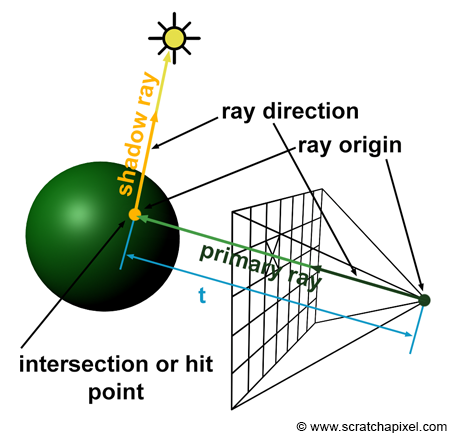
\includegraphics[width=\linewidth]{pinhole_camera.png}
  %\captionsetup{   width=.5\linewidth}
  \caption{A pinhole camera inside a scene with a sphere and a light source}
  \label{fig:pinhole}
\endminipage\hfill
\minipage{0.54\textwidth}
  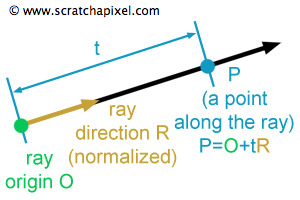
\includegraphics[width=\linewidth]{ray.png}
  \caption{Ray model}
  \label{fig:ray}
\endminipage
\end{figure}

A ray is defined as a point and a direction, as shown in \autoref{fig:ray},
in formulas:
$$
r(t) = O + tR
$$
where $O,R \in \R^3$ and $R$ is a unit vector.
At each time $t$ we can compute a point position on the ray, in this way the ray tracing algorithm can check for each $t$ whether the ray intersected a surface or not.
%Obviously we also need to take in consideration the machine precision and the time limits, but 

%Until know we 
%Because the ray origin and direction depends respectively on the camera's position and the camera's orientation, we need a method to 

When generating rays we have to take in consideration several factors:
camera position and orientation are the more obvious, but also the field of view and the image aspect ratio.
%Actually there are more 
First of all we need to derive the rays' direction with the pixel's centers on the image plane (the rectangle with a grid) and the camera origin (also called \emph{eye}).
But these two values refers to different coordinate systems because the pixel position refers to the top left corner of the image plane and the camera origin is defined in world coordinates.
Here with world coordinates we mean the coordinate system with which the object (and the camera) are placed on the scene.
One way to solve this problem is to produce the rays as if the camera was placed in the origin looking towards $-z$ and then transate and rotate the rays according to the true camera position and orientation.

In order to do so we need to remove the dependency from the actual output image size.
Given two coordinates in raster space we normalize them by dividing respectively by the image width and height.
Now the coordinate are in Normalized Device Coordinates (NDC) space.
Actually the precise operation is the following, in which we also move the coordinate in pixels center:
\begin{align*}
  PixelNDC_x &= \dfrac{(Pixel_x + 0.5)}{ImageWidth}\\
  PixelNDC_y &= \dfrac{(Pixel_y + 0.5)}{ImageHeight}
\end{align*}
Now we have to map this coordinates form $[0,1]$ into $[-1,1]$ because the eye of the camera is at the origin, so the center of the image plane (also called screen) is on the $z$-axis.
In practice we are aligning the sign of the four quadrants of the $xy$-plane in world coordinates with the image plane.
\begin{align*}
  PixelScreen_x &= (2 * PixelNDC_x - 1) * AspectRatio\\
  PixelScreen_y &= 1 - 2 * PixelNDC_y
\end{align*}
Remember that we want a right handed system so we map:
the top left corner, $(0,0)$ in raster space, to $(-1,1)$ in screen space;
the bottom right corner, $(ImageWidth,ImageHeight)$ in raster space, to $(1,-1)$ in screen space; and the last two accordingly.

The $AspectRatio$ used in the formula equals $ImageWidth / ImageHeight$ and we must consider it when the output image is not squared.
In fact we need to produce more pixel in one direction otherwise the generated image will look squished.

One of the last thing to consider is the field of view (fov), the view angle of the camera.
Assuming that the distance between the camera eye and the image plane equals to $1$, we want to know by how much enlarge or shrink the image plane horizontally and vertically.
Knowing the fov angle $\alpha$ we just need to multiply the screen coordinates by $\tan(\alpha/2)$.

The last thing to take in consideration is that out camera may not be always positioned in the world origin and look toward $-z$.
To do so there are several options the one explained here is also 
\todo[inline]{explain like if we are moving a point with a normal direction}





\subsection{Sphere Tracing}
Introduced by Hart\cite{hart1996} in 1996, the sphere tracing algorithm gives a better alternative to other ray tracers like ray marching.
In ray marching each ray is analyzed by constant steps of $t$.
We can detect a ray-surface contact using the sign of the distance function: when the ray enters the surface the distance became negative.
Let's say that for a ray $r$, $d(r(t_k),S) > 0$ and $d(r(t_{k+1}),S) < 0$, for some instant $t_k$ and the following instant $t_{k+1}$ and an implicit surface $S$.
Then using bisection on the segment between the two points $r(t_k)$ and $r(t_{k+1})$
we look for the point $P$ on the segment for which $d(P,S) = 0$.
To actually find this point $P$ on the surface $S$ can be costly, so usually it's found a point that is as near to the surface as a given threshold.

We can speed up the algorithm by increasing the step size, i.e. $t_{k} - t_{k+1}$, but doing so leads two problems:
performing bisection is slower because the segments are longer;
if an object is small the algorithm may evaluate the ray just before and after the object, thus not seeing it.
While the first problem can be managed, the second can cause completely wrong images to be produced.
What we would like is an algorithm with an adaptable step size, to go fast when there are no surfaces near and to slow down when there are objects in the proximity: sphere tracing does that.

Remember that before we said that $d(x,S)$ for some $x \in \R^3$ means we can move $x$ in every direction by $d(x,S)$ being sure at worst to just hit the surface.
In other words we are drawing a safe sphere around the point, in which there is no surface.
%If we evaluate the distance metric for each surface in the scene and take the minimum 
Form the surface perspective this sphere is called an \emph{unbounding sphere}\cite{hart1996}, and the union of all the unbounding spheres describes the surface because no sphere penetrate the object.
The concept is approximately the opposite of \emph{bounding volume}, a volume that surrounds the object, because here we define an area of space not containing the object.
In sphere tracing the ray-surface intersection is determined by a sequence of unbounding spheres, as shown in \autoref{fig:hit_and_miss}.
\begin{figure}[!htb]
\minipage{0.40\textwidth}
  \begin{lstlisting}
  t = 0
  while (t < D) {
    d = f(r(t))
    if (d < $\epsilon$) {
      // intersection
      reutrn t
    }
    t += d
  }
  // no intersection
  return $\emptyset$
  \end{lstlisting}
  \caption{Pseudo code for the geometric implicit surface rendering algorithm}
  \label{pscode:sphere_tracing}
\endminipage\hfill
\minipage{0.59\textwidth}
  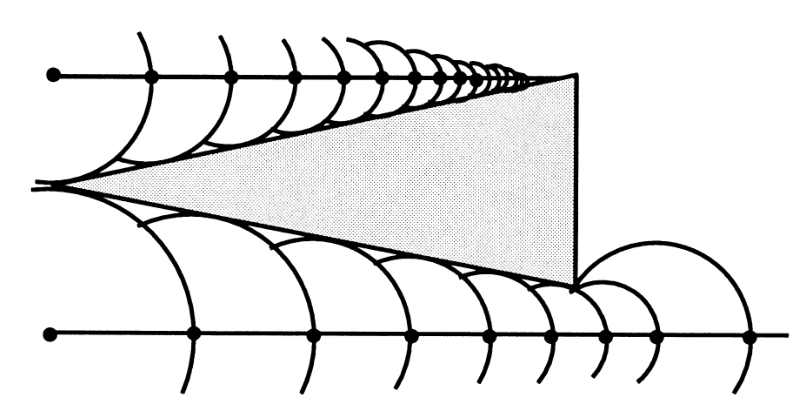
\includegraphics[width=\linewidth]{hit_and_miss.png}
  \caption{A hit and a miss (image from \cite{hart1996})}
  \label{fig:hit_and_miss}
\endminipage
\end{figure}

The pseudo algorithm for rendering one implicit surface is listed in \autoref{pscode:sphere_tracing}.
In the pseudocode $D$ is the maximum ray traversal distance, $\epsilon$ is the minimum distance from a surface to consider a hit, $t$ and $r(t)$ are the usual ones and $f$ can be a DIF or a DUF.
As said before the DUFs are ``more cautious" because are a lower bound to the maximum distance traversable without hitting the surface.
When we can't use the exact signed distance function of the surface we can use safely its bound, knowing that the convergence will be slower because the algorithm will make more steps.
The following theorem from \cite{hart1996} shows that the speed drop is negligible because the algorithm is still linear even if we are using a signed distance bound.
We look at sphere tracing as a root finding algorithm.
\begin{theorem}
Given a function $f: \R \to \R$ with the Lipschitz bound $\lambda \geq Lip(f)$ and an initial point $t_0$, sphere tracing converges linearly to the smallest root grater than $t_0$.
\end{theorem}
\begin{proof}
  We can write the sphere sequence as
  \begin{equation}\label{eq:st_seq}
  t_{i+1} = g(t_i) = t_i + \dfrac{\abs{f(t_i)}}{\lambda}
  \end{equation}
  %https://en.wikipedia.org/wiki/Newton%27s_method
  to emphasize the similarities with the Newton's root finding method.
  Let $r$ be the smallest be the smallest root greater than the initial point $t_0$.
  Since $f(r) = 0$, then $g(r) = r$, and at any non root $\abs{f(t_i)}/\lambda$ is positive.
  Hence \autoref{eq:st_seq} converges to the first root.
  Without loss of generality we assume $f$ to be non-negative in the region of interest, eliminating the need for the absolute value.
  %https://en.wikipedia.org/wiki/Taylor_series
  The Taylor expansion of $f(t_i)$ about the root $r$ is:
  \begin{equation}\label{eq:st_taylor}
    g(t_i) = g(r) + (t_i - r) g'(r) + \dfrac{(t_i - r)^2}{2} g''(\tau)
  \end{equation}
  for some $\tau \in [t_i, r]$ and $g'(r) = 1 + f'(y)/\lambda$.
  The error term becomes:
  \begin{align*}
    e_{i+1} &= t_{i+1} - r = g(t_i) - g(r) =\\
            &= g'(r)e_i + \text{higher-order terms}
  \end{align*}
  Since $g'(r)$ is constant in the iteration \autoref{eq:st_seq} converges linearly to $y$.
\end{proof}
\begin{corollary}
  Sphere tracing converges quadratically if and only if the function is steepest at its first root.
\end{corollary}
\begin{proof}
  In the event that $f'(r) = - \lambda$, the linear term of the error of \autoref{eq:st_taylor} drops out, leaving the quadratic and higher-order terms.
\end{proof}

One thing to highlight is about the rays that pass near a surface without hitting it.
Such rays will slow down because their distance to the surface becomes smaller and smaller until theyy pass over it, as shown in \autoref{fig:hit_and_miss}.
This effect can be seen in practice coloring the pixels with respect to the number of steps the ray had to do before hitting something or traversing the maximum distance.

\todo[inline]{generate image with pixel colored according to steps num}
\begin{figure}[!htb]
  \centering
  %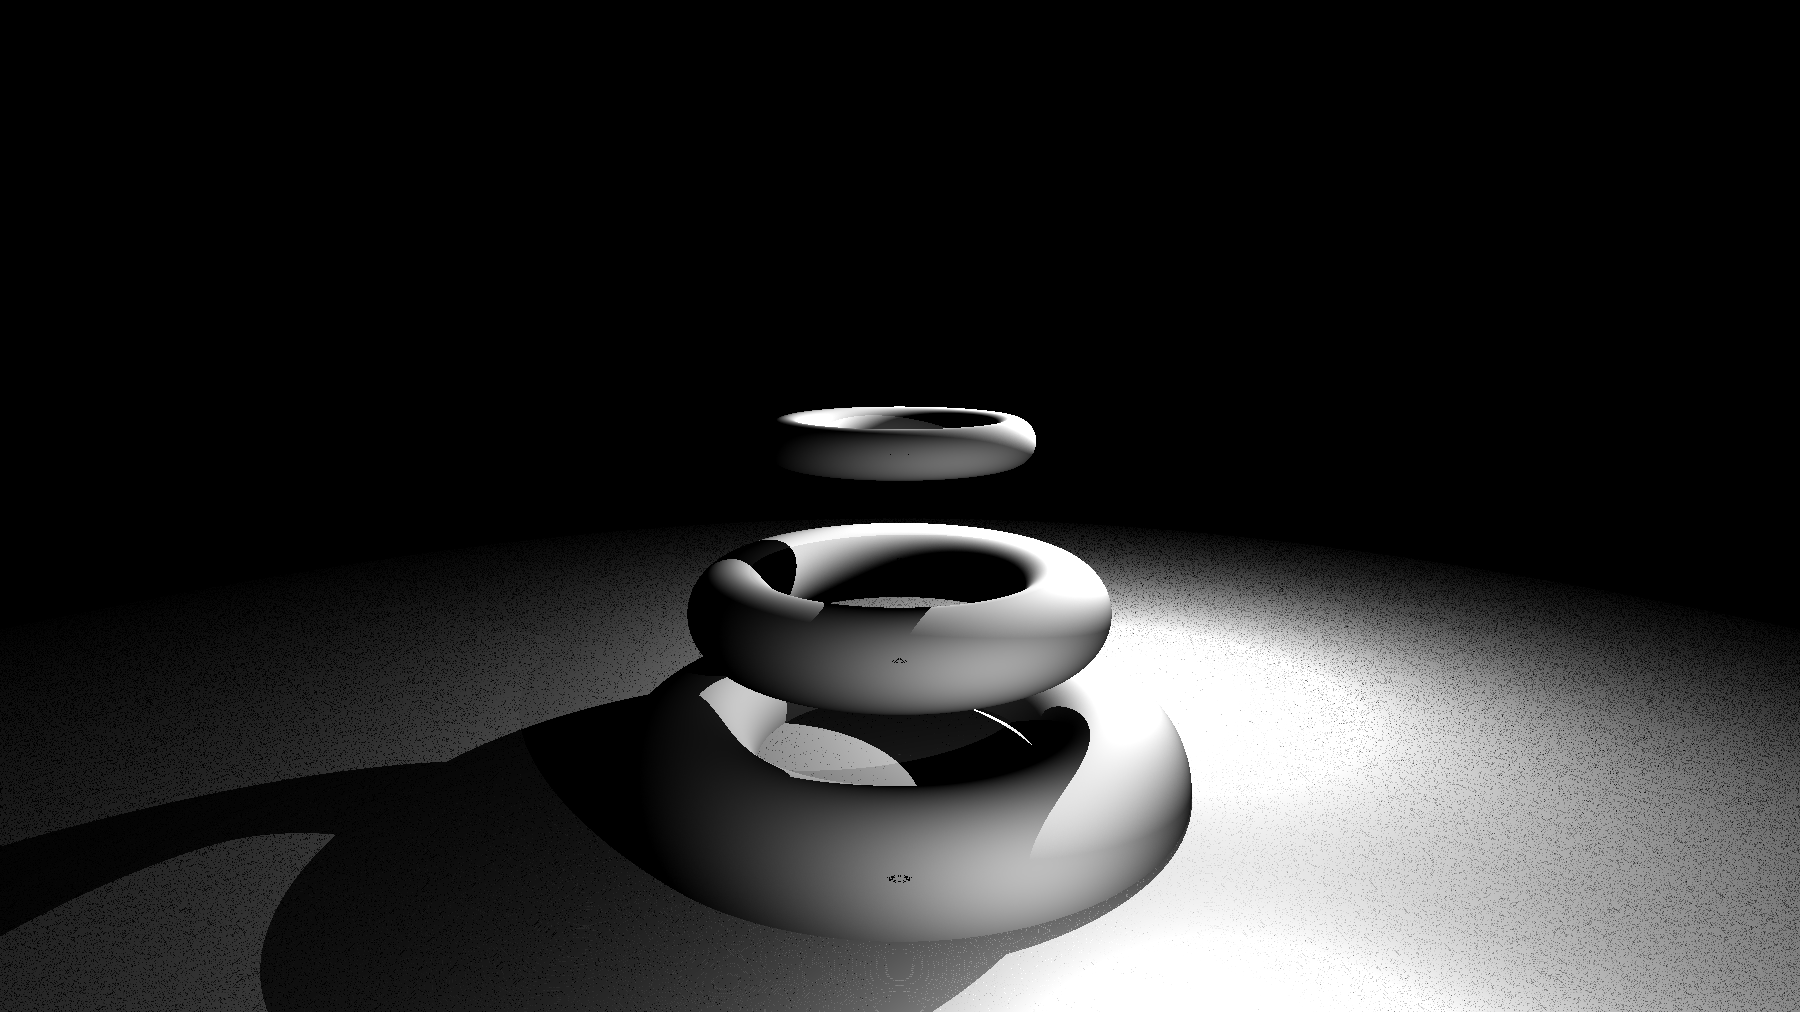
\includegraphics[width=\linewidth]{img_02.png}
  \includegraphics[width=.8\linewidth]{example-image-a}
  %\caption{TODO}
  %\label{fig:union}
\end{figure}






%\subsection{Shading and Lightning}
\subsection{Lightning and Shadows}

%In computer graphics, a shading function is defined as a function which yields the intensity value of each point on the body of an object from the characteristics of the light source, the object, and the position of the observer. Phong - 1975.

%To compute properly the color of surface lighted by a ray of light at least we need 

Shading is a complex field and here we address only the problem of computing simple lighting and hard shadows, leaving for future improvements topics as non punctual lights, reflection, refraction, and semi-transparent objects.

Even in this simplified setting we need to compute the surface normal at a point, 
that's because we need to know the quantity of light that the point receives, i.e. If the surface is facing or not the light source.
Because we are handling implicit functions we can't rely on already existing information, as happens with ``classic" rendering and \emph{.obj} files for example.
We need to compute the surface's normal at a point with only its implicit definition.
To do so we can take advantage of the gradient of the function.
Remembering that the gradient is the rate-of-change of the function over a direction, given $f$ we want to compute the gradients with respect to $(1,0,0)$, $(0,1,0)$ and $(0,0,1)$.
These results combined will form a 3D vector, which after being normalized becomes the normal we are looking for.

More formally, we define $\nabla f$ as the gradient of the implicit function $f(x,y,z)$ and let $P = \left< x_0, y_0, z_0 \right>$ be a point on the surface, thus $f(x_0, y_0, z_0) = 0$.
All we need to do is to observe the rate-of-change in the proximity of $P$,
this can be done numerically with 
\begin{align*}
  \nabla f_{x_0} &= f(x_0+\delta, y_0       , z_0       ) - f(x_0-\delta, y_0       , z_0)\\
  \nabla f_{y_0} &= f(x_0       , y_0+\delta, z_0       ) - f(x_0       , y_0-\delta, z_0)\\
  \nabla f_{z_0} &= f(x_0       , y_0       , z_0+\delta) - f(x_0       , y_0       , z_0-\delta)\\
  \nabla f   &= \left< \nabla f_{x_0}, \nabla f_{y_0}, \nabla f_{z_0} \right>
\end{align*}
The following steps assure us that $\nabla f$ has actually the normal's direction.
First we define
$$h(t) = \left< x(t), y(t), z(t) \right>$$
to be a parametric definition of a curve that lies on the surface and that passes through $P$.
We also define 
$$g(t) = f(h(t)) = 0$$
Note that exists a particular $t_0$ such that
$$g(t_0) = f(h(t_0)) = f(x(t_0), y(t_0), z(t_0)) = f(x_0, y_0, z_0) = f(P)$$ %%f(x_0, y_0, z_0) = 0$$
Now we can calculate the gradient at 
\begin{align*}
  \dfrac{dg}{dt} &=
\dfrac {\partial f} {\partial x} \bigg\rvert_{P} \dfrac {d x} {d t} \bigg\rvert_{t_0} + \dfrac {\partial f} {\partial y} \bigg\rvert_{P}\dfrac {d y} {d t} \bigg\rvert_{t_0} + \dfrac {\partial f} {\partial z} \bigg\rvert_{P}\dfrac {d z} {d t} \bigg\rvert_{t_0}
=\\
                 &= \left< \dfrac {\partial f} {\partial x} \bigg\rvert_{P}, \dfrac {\partial f} {\partial y} \bigg\rvert_{P}, \dfrac {\partial f} {\partial z} \bigg\rvert_{P} \right> \cdot \left<  \dfrac {d x} {d t} \bigg\rvert_{t_0}  \dfrac {d y} {d t} \bigg\rvert_{t_0}  \dfrac {d z} {d t} \bigg\rvert_{t_0} \right> = 0 %\\
%\leftrightarrow \nabla f|_P \cdot r'(t_0) = 0.
\end{align*}
The equation comes from the higher dimensions version of the chain rule $g'(t) = h'(t) \cdot f'(g(t))$.
The vector form comes from $a \cdot b = a_x b_x + a_y b_y + a_z b_z$, and highlight the perpendicularity between the two vectors.

Now that we have the surface normal $N$ at $P$ we can use it inside a rendering equation that, in simple words, gives the amount of light reflected by the surface.
Putting in formulas
$$
\dfrac{ (n \cdot l) c_{light} }
{ 4 \pi }
$$
where $n$ is the surface normal, $l$ a unit vector pointing the light and $c_{light}$ its color.
Remember that the dot product $n \cdot l$ gives the cosine of the angle of indicente of the light rays.
The denominator comes from the solution of an integral over a hemisphere centered in $P$, more on shading in \cite{real_time_rendering}.
If there are more light sources we can just iterate over them and sum the contribution of each.
We can also consider adding an ambient light to give a minimum lighting to all the surfaces, thus removing the completely black areas from the image.

For what concerns shadow we can just cast a second ray from $P$ towards a light.
We follow the ray until we hit either a surface or the light itself:
in the first case we just stop computing this light's contribution to the shading of $P$ (its contribution is equal to zero because no light ray can reach the point);
in the second we procede as described before.
The ray can be computed with a modified version of the sphere tracing algorithm that stops at the first surface hit.
\begin{figure}[!htb]
  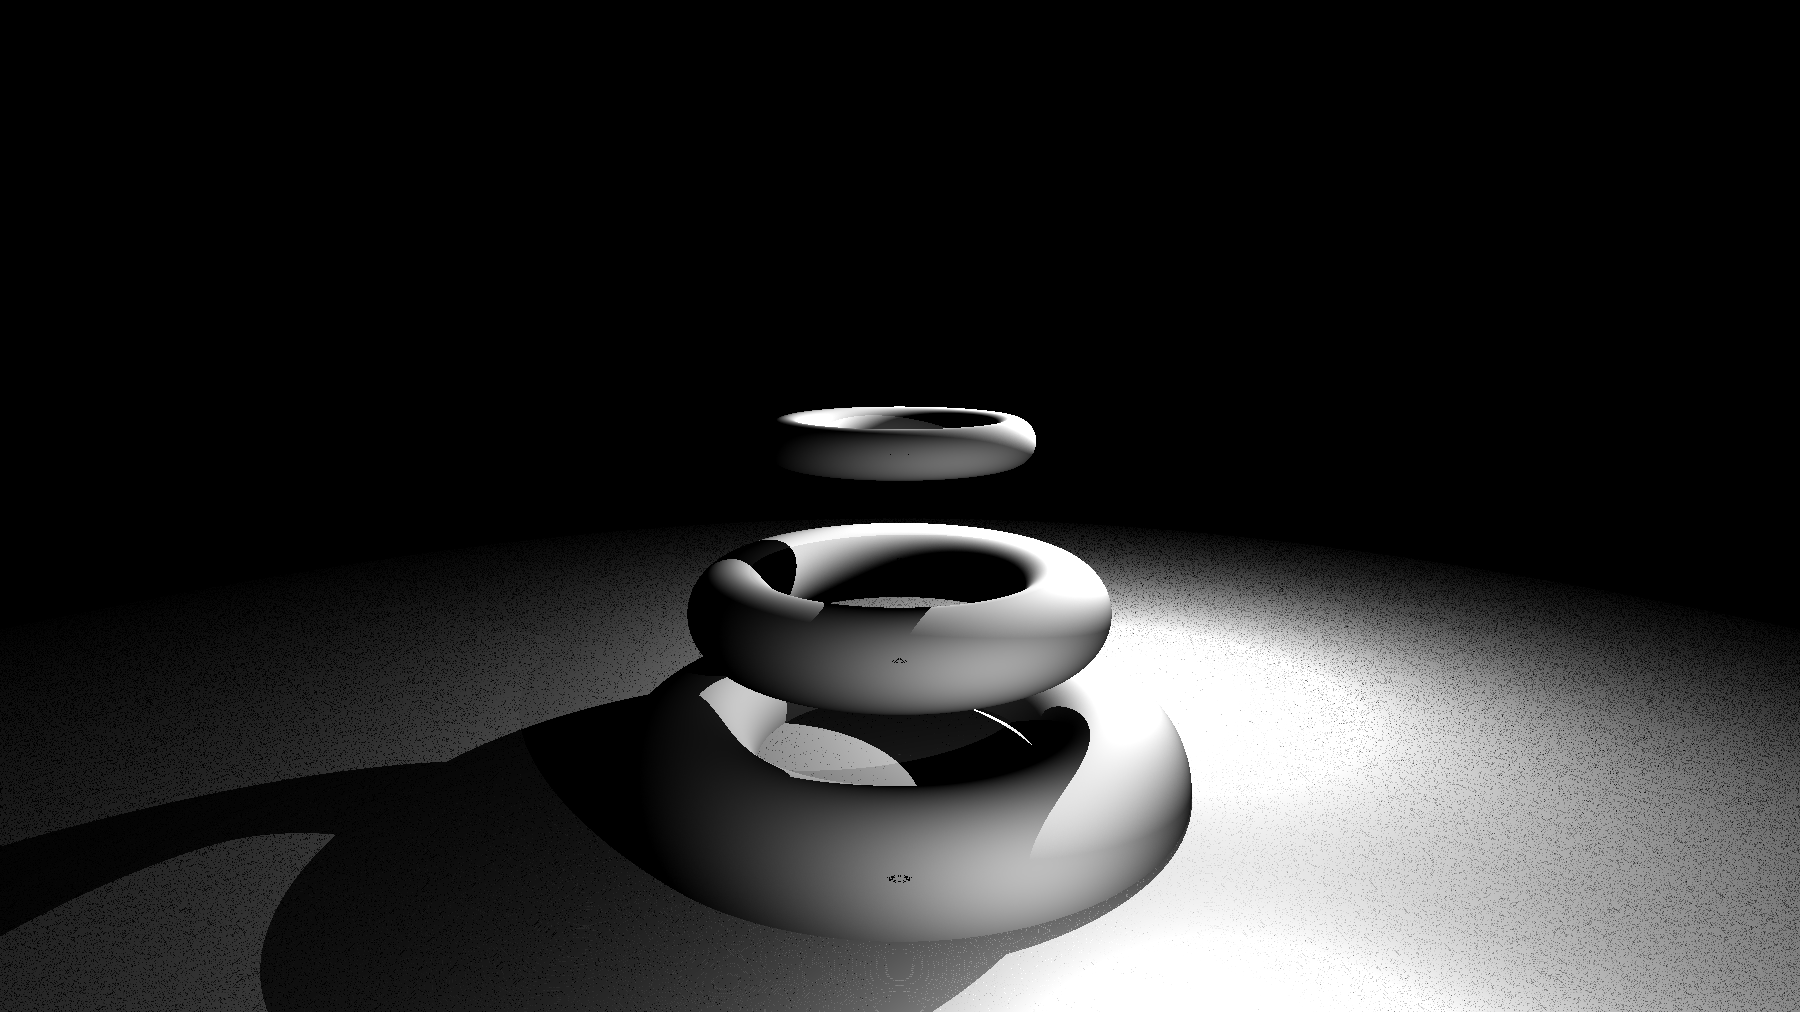
\includegraphics[width=\linewidth]{img_02.png}
  \caption{A scene with 3 torus, a big sphere (the terrain) and two point lights rendered with hard shadows and no anti-aliasing.}
  %\label{fig:union}
\end{figure}

\subsection{Anti-Aliasing}
\todo[inline]{re-read hart1996 and scratchpixel on cone tracing}

\begin{itemize}
  \item what is and why we cannot remove it completely from RayTraced imgs \cite{rt_groundup}

%% Scratch Pixel notes
  \item simple method: supersampling as described and implemented in \cite{rt_one_weekend}
  \item in \cite{hart1996} proposes an interesting method that takes advantage of sphere tracing algorithm nature.




\end{itemize}
